% Caractéristiques types d'un paragraphe:
% \subsection{TitreDuParagrape}
% \subsubsection{Description}
% \hypertarget {titreduparagraphe} (en minuscule et sans accent)
% Votre texte
% \subsubsection{Personalités} (si besoin est)
% Merci de retourner à la ligne à chaque phrase. Cela n'influencera pas la présentation de votre texte et permettra une meilleure lisibilité
% Un lien intra document se fait ainsi: \hyperlink {lenomdepuaragraphe (tel que déclaré via hypertarget)}{le texte à afficher}
% Merci de votre participation à Creare Mundum ;)

\section{Kazadren}
\subsubsection{Description}
\hypertarget{kazadren}{}Littéralement maison de Dren cette chaine de montagnes, au nord de l'empire humain, renferme un des plus grand royaume nain de ce monde.
Elles regorgent de minerais et de pierres précieuses. Elles sont actuellement dirigées par Folii, roi sous la montagne.
Sa capitale est Dren, où réside Folii. Ces montagnes sont remarquablement froides et toujours recouvertes de neige. 
Ces montagnes sont aussi prodigieusement riches en minerais de toute sorte. 
L'extrémité ouest est inhabitée car fouettées en permanence par des vents violents.
\subsection{Les arodefs}
\subsubsection{Description}
L’arodef est une sorte de croisement entre un cheval, un rhinocéros et un mammouth. Il pèse dans l’ordre de 500 kilos et mesure d’un mètre vingt à un mètre cinquante pour les plus hauts. Il possède un pelage laineux, ainsi que plusieurs cornes sur le museau et autour du cou. Les arodefs vivent dans dans de longs tunnels sous terre, juste assez profond pour manger les racines des arbres. Du fait de leur vie souterraine, les arodefs sont à peu près aveugles, mais leurs autres sens sont sur-développés. Il vont donc principalement se déplacer grâce à leur ouïe, leur odorat et leur sens du toucher. Ce sont les seules montures à pouvoir se déplacer de jour comme de nuit, bien qu’ils soient assez lents. Les arodefs sont beaucoup utilisés pour les transport ainsi que pour la guerre. Ils sont effet très résistants et combatifs. Ce dessin d’un arodef de guerre avec son cavalier vaut mieux que de longues descriptions (bien que l’arodef présent ait un air particulièrement haineux). 
\begin{figure}[ht]
\begin{center}
   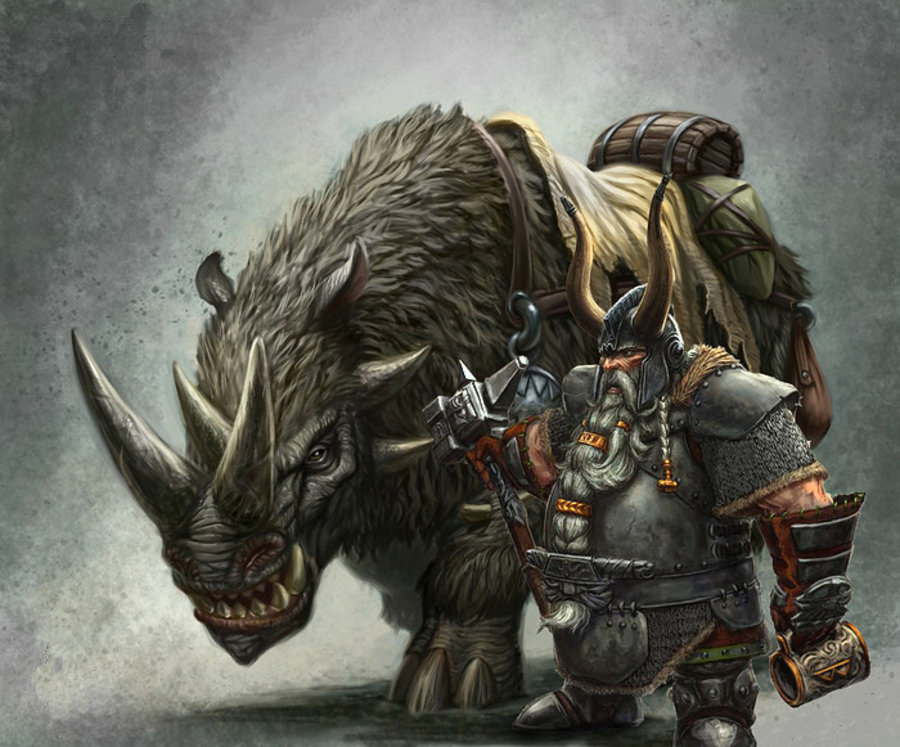
\includegraphics[scale=1.2]{./Ressources/medieval/arodef.jpg}
   \caption{Un arodef de guerre}
\end{center}
\end{figure}
\subsubsection{Histoire}
Présent depuis longtemps sur les cimes des montagnes, les arodefs ont été domestiqué par le peuples nain. Ces derniers s’en servent essentiellement en tant que monture, que ce soit de voyage ou de guerre. 
\subsubsection{Élevage}
Les arodefs sont élevés par le peuple nain dans les salles les plus hautes, afin que les bêtes puissent manger leur racines. Les palefreniers nains sont très réputés de part le monde. 
\subsection{Dren}
\subsubsection{Description}
\hypertarget{dren}{}Capitale du royaume nain de Folii, peu de gens ont eu la chance de la voir.
Elle est cachée dans les sommets brumeux de Kazadren.
Le petit nombre de personnes qui y sont rentré la dépeigne superbe, magnifique et immense.
Les murs seraient même couverts d'or! 
Elle renferme un des plus gros filon d'or du monde connu.
Les trésors qui y sont entreposés ont attirés bien des convoitises, mais les rois nains ont toujours su les garder.
Peu de marchands s'y rendent, en effet, pour y rentrer, il faut qu'un nain de Dren vous y invite, sinon la porte reste close.
C'est pourquoi Sombre-Cime a été construite, pour servir d'intermédiaire entre les nains de Dren et les Hommes.
\subsubsection{Accès}
Pour parvenir à la belle Dren, il faudra suivre une longue route qui serpente à flan de montagne. Elle se termine net devant une paroi rocheuse. Il faut alors attendre qu'un résident décide de vous laisser rentrer, les portes ne s'ouvrant que de l’intérieur. Une fois l'ordre donné, le mur s'ouvre, comme par magie, suivant des contours invisible à l’œil nu. La porte fait environ deux mètres d'épaisseur, et est taillé à même la montagne, c'est une prouesse technique et artistique, l'intérieur étant somptueusement décoré.
\subsubsection{Les résidents}
Ce titre permet bien des choses à celui qui le porte dans le territoire nain, ainsi qu'un grand respect. Il est automatiquement accordé aux propriétaires des maisons de Dren, et est lié à ces maisons. Il suffit de porter la clé (unique, chef d'oeuvre du savoir faire nain), pour avoir accès aux privilèges de ce titre. Ils sont:
\begin{itemize}
\item Le droit de faire entrer quelqu'un en ville (le détenteur en prends alors l'entière responsabilité).
\item Le droit de siéger aux banquets du roi.
\item Un accès complet à tout le territoire nain des montagnes de Kazadren.
\item Un droit de parler pour les questions concernant la ville.
\item Un coffre à la banque royale.
\end{itemize}
\subsubsection{Personalités}
\paragraph{Folii}
\hypertarget {folii}{}Roi sous les montagnes de Kazadren, il dirige avec aisance et bonté sa somptueuse capitale, Dren.
Folii est petit et corpulent (du moins, plus que la normale chez les nains).
Il est beaucoup aimé de son peuple et des hommes. Il est à l'origine de la construction de \hyperlink {sombrecime}{Sombre-Cime}, pour une meilleur communication entre nain et hommes. 
C'est un fervent opposant de Dwali, car pour un libéralisme des nains.
\subsubsection{Relations}
\begin{itemize}
\item Aegnord: Aucune relation, Méfiant 
\item Anksfall: Commerce, Bonne relation 
\item Grahyrst: Assez bonne relation 
\item Ketelundr: Hostile 
\item Leheath: Assez bonne relation
\item Mauhagr: Méfiant 
\item Rinam: Aucune relation, En paix
\item Sombre-Cime: Commerce, Très bonne relation 
\item Thorneye: Aucune relation, Méfiant 
\item Vrag: Commerce, Méfiant 
\end{itemize}
\subsection{Dûn Antil}
Dûn Antil est en langue naine et signifie ’Vieux château’ en commun. Depuis longtemps inhabité, Dûn Antil est une ancienne place forte naine, du temps de leur possession des plaines de sang. Elle se trouve sur les contre-forts des montagnes de Kazadren. Elle fut détruite par les nains, ne voulant pas laisser une telle place forte aux humains lors de leur départ de ces terres. C’est un lieu oublié et peu de personnes s’y rendent. 
\section{Les zones à influences humaines}
\subsection{Sombre-Cime}
\subsubsection{Politique}
Sa construction a été ordonée par Ermudor lui même, qui shoutait un rapprochement avec les nains du nord à la sortie de la guerre. Elle fut achevée en l'an 552. Elle restat un duché de l'empire jusqu'a l'explosion de ce dernier.
\newline
Depuis, Sombre-Cime est la capitale du royaume humain du nord. Le dirigeant de la ville a néanmoins gardé le titre de "Duc".
\subsubsection{Description}
\hypertarget{sombrecime}{}Perchée sur les hauteurs de Kazadren, cette ville fait office d’ambassade humaine auprès des royaumes nains. Sombre-Cime est aussi un exemple de diversités, nains, hommes, orques, elfes, toutes les races y sont représentées. Sombre-Cime est aussi très réputée pour sa foire annuelle, puisqu’elle regroupe les meilleurs artisans nains et humains. Un épais brouillard y règne une grande partie de l’année. La ville est actuellement dirigé par le duc Lasym, qui est bon et juste.
\begin{figure}
 \begin{center}
   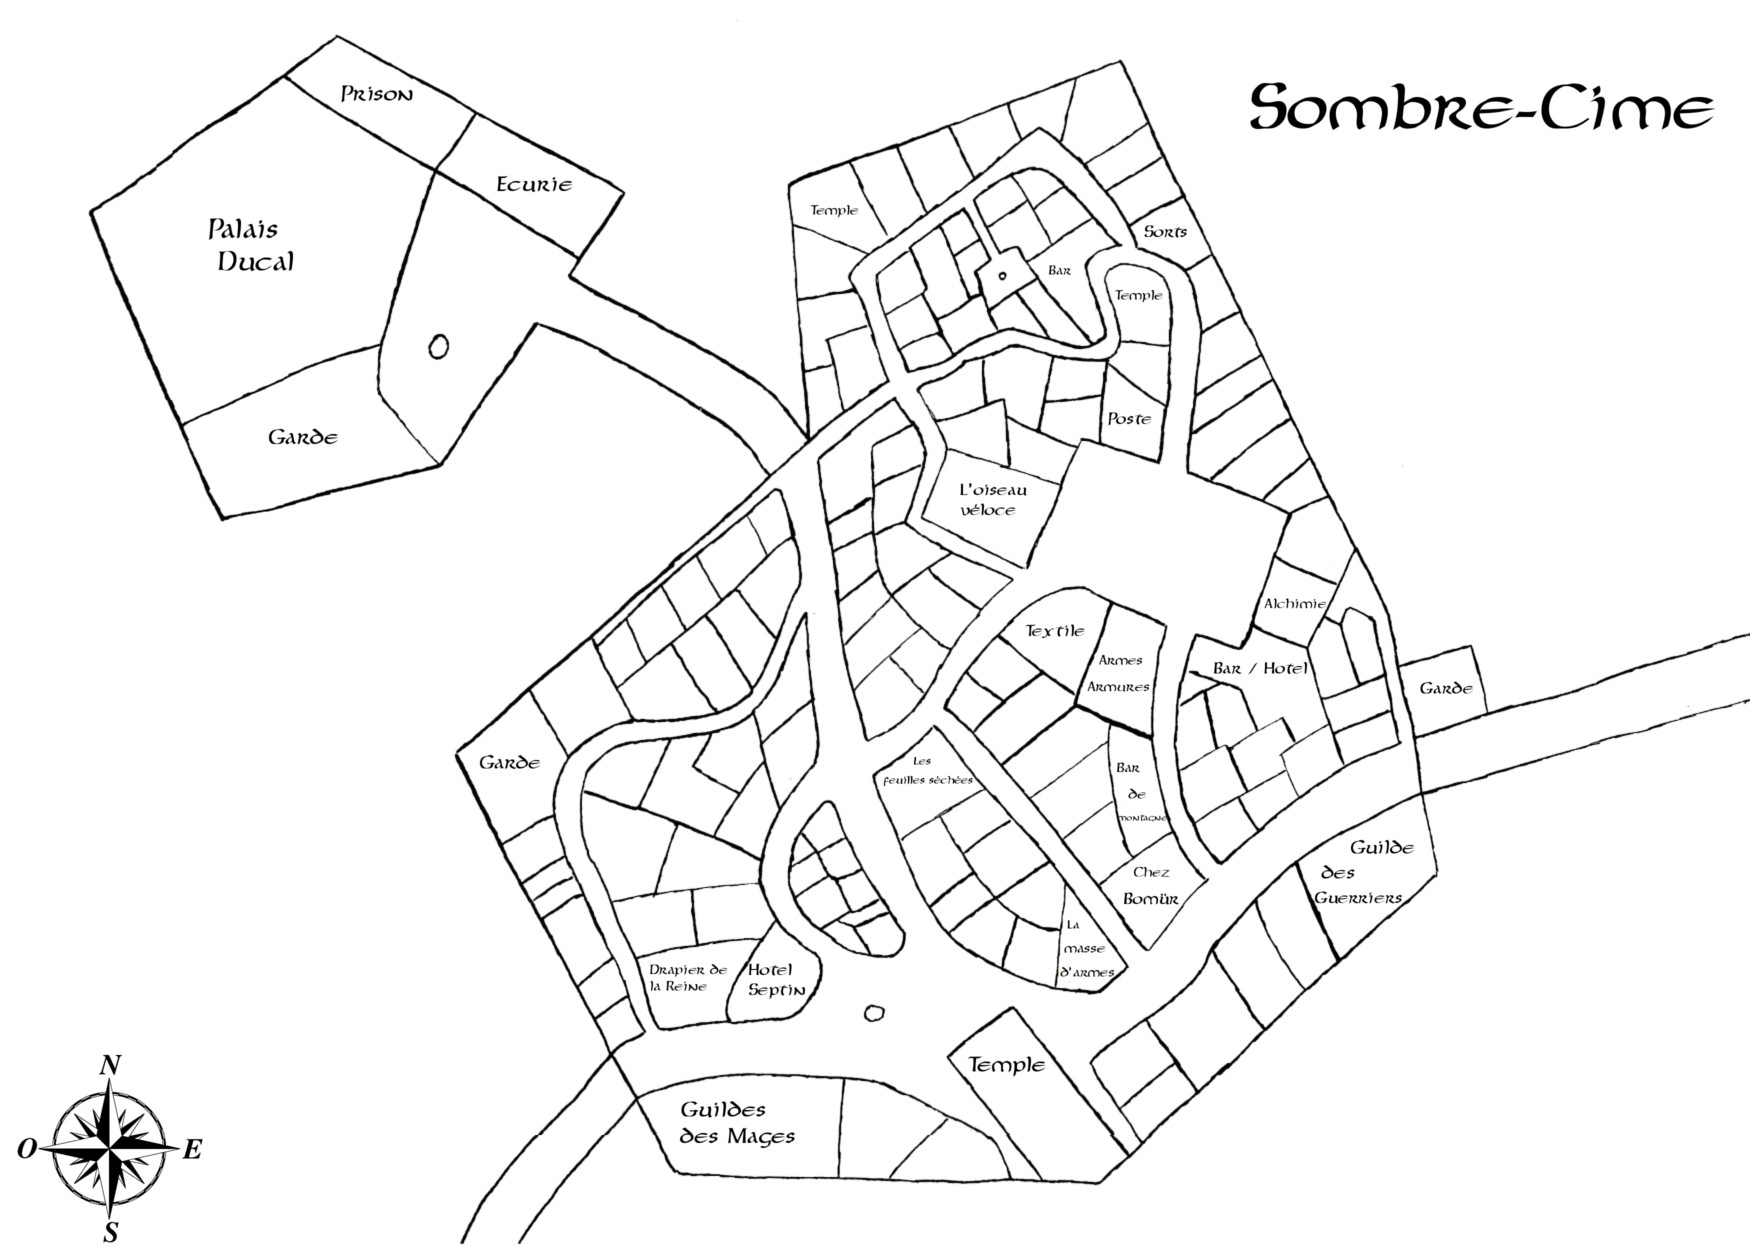
\includegraphics[scale=1.14, angle=90]{./Ressources/medieval/Carte_sombre_cime.jpg}
   \caption{Carte de Sombre-Cime en l'an 512}
 \end{center}
\end{figure}
\subsubsection{Population}
Sombre-Cime est une ville assez cosmopolite, car elle est à la croisée de plusieurs pays.
Il y a environ 45\% d'humains, 35\% de nains, 15\% de barbares, et 5\% de divers peuples.
\subsubsection{Ambiance}
La ville de Sombre-Cime est, comme son nom l'indique, pas très joyeuse. 
Les températures rigoureuses, ainsi que les vents violent expliquent en partie cette morosité ambiante.
Mais, une semaine par an, lors de la grande foire, Sombre-Cime devient une des villes les plus agréable de l'empire!
Les maisons et les rues sont faites en bonne pierres de taille, ce qui en fait une ville assez belle.
La vue est assez magnifique sur les plaines de sang. 
Mais le brouillard quasi-permanent empêche de profiter du paysage.
\subsubsection{Lieux}
\paragraph{Chez Bömur}
Bömur est un descendant de nain et d'humain. 
Il tient sa petite auberge seul, sa femme ayant été emportée par la fièvre.
Beaucoups d'habitants de Sombre-Cime aiment s'y retrouver une fois la nuit, et la brume, tombées sur la ville.
Son auberge est relativement petite, il n'y a que  chambres, mis Bömur a une grande salle où il tiens son bar et sert son diner.
Il fait tout lui-même.
\paragraph{Les feuilles séchées}
Les feuilles séchées est une petite boutique d’alchimie, tenue par Mme. Liro, une vieille femme humaine. Une forte odeur de lavande règne perpétuellement dans l’air vicié de la boutique. Son stock est relativement bon, et tout petit herboriste y trouve son bonheur. 
\subsubsection{Les guildes}
\paragraph{La guilde des guerriers}
La guilde des guerriers est dirigé par le duc Lasym en personne. De ce fait, elle est assez apprécié et jouit d’une aide sans réserve de la garde de la ville.
\paragraph{La guilde des mages}
La guilde des magiciens est dirigée par un mage de petite renommée depuis longtemps aveugle. Elle n’est pas encore très bien acceptée, les nain étant assez hostile à ce genre de pratique. 
\subsubsection{Personalités}
\paragraph{Tasach Lasym}
Premier duc de Sombre-Cime, il d'abord servit longtemps dans l'armée, sous le grade de général.
Puis, une fois à la retraite, l'empereur lui a offert le nouveau duché de Sombre-Cime.
Il l'administrait avec bonté et bienveillance.
Le duc était relativement âgé, environ 50 ans et plutôt de grande stature.
Il arborait fièrement une barbe blanchissante.
Il possèdait une balafre sur la joue, souvenir d'un adversaire plutôt téméraire.
\subsubsection{Relations}
\begin{itemize}
\item Aegnord: En paix 
\item Anksfall: Commerce, Très bonne relation 
\item Dren: Commerce, Très bonne relation 
\item Grahyrst: Excellente relation  
\item Ketelundr: Aucune relation, Méfiant
\item Leheath: Commerce, Assez bonne relation 
\item Mauhagr: Hostile, Inspire la peur 
\item Rinam: Aucune relation, En paix 
\item Thorneye: Assez bonne relation 
\item Vrag: Assez bonne relation 
\end{itemize} 
\subsection{Les Plaines de Sang}
\subsubsection{Description}
\hypertarget{lesplainesdesang}{}
Les plaines de sang sont le grenier des humains. Un blé rouge y pousse, et, vu de des montagnes de Kazadren, les plaines sont semblables à des rivières de sang.
\subsection{Légendes}
Voir la note n\degre236, la chute de Dolgarur, par Milan de Garabe.
\subsubsection{Personalités}
\paragraph{Dolgarur}
\hypertarget {dolgarur}{}Dolgarur fut un des rois nains les plus respectés de l'histoire, mais il sombra dans la folie, sous l'emprise d'un mystérieux sort. 
Il se mit alors en guerre contre les elfes. 
Il mourut sur le champ de bataille des Plaines de Sang.
\subsection{Darkhaven}
\subsubsection{Description}
\hypertarget{darkhaven}{}Cette sombre forêt a longtemps été réputée maudite,
mais c'est sans doute \hyperlink{laguildedesvoleurs}{la guilde des voleurs} qui fait courir ce bruit pour décourager les intrus.
Elles abrite le quartier générale de la guilde des Voleurs, ainsi que la racine de de leur salle de communication. 
On dit que n'importe quel voleur peut y entrer, les autres se font tuer dès qu'ils posent un pied dans la forêt.
\subsection{La Mer Intérieure}
\subsubsection{Description}
\hypertarget {lamerinterieure}{}Cette mer d'huile est sans danger.
Il arrive cependant qu’elle se mette en furie et elle fait alors de monstrueux ravage.
Ce phénomène est inexpliqué à ce jour.
Beaucoup de petit village de pécheur l'entoure.
\subsection{Le grand fleuve}
Le Grand Fleuve sépare littéralement l'empire en deux. Il prend ses sources dans les sommets des montagnes de Kazadren, puis descend jusqu'à Darkhaven, se jette dans la mer intérieure pour ensuite traverser Grahyrst et enfin se jeter dans la mer.
\subsection{Anksfall}
\subsubsection{Description}
\hypertarget{anksfall}{}Capitale de l'empire humain, cette ville est réputée pour sa grande beauté,
notamment le grand dôme qui surplombe le palais de l'empereur. 
La ville est divisée en deux grandes parties: La Haute-Ville 
(où loge l’empereur, le duc d'anksfall, les bourgeois et les notables)
et la Basse-Ville qui regroupe tout les quartiers pauvres et le port.
Il ne fait pas bon y aller une fois la nuit tombée.
Ces quartiers abriteraient même une des salle de communications de \hyperlink {laguildedesvoleurs}{la Guilde des voleurs}.
\subsubsection{Hiérarchie}
En haut de toute l'organisation sociale se trouve bien évidement l’empereur, puis vient le duc d’Anksfall, traditionnellement son fils. En l’absence d’un héritier de la couronne, la place est assuré par un membre de la famille impériale. C’est à ce dernier que revient l’administration de la ville, l’empereur s’occupant de choses plus importantes que les menus problèmes de la cité. La suite reprend le modèle classique d’une ville. 
\subsubsection{Le Festival d'Anksfall}
Tous les ans à Anksfall se tient une célébration reconnue dans tout le pays et même au-delà comme un évènement des plus spectaculaires de ce monde. Créé à l'origine pour fêter l'arrivée de la nouvelle année et par conséquent les nouvelles semailles, le festival est une occasion pour tous de se changer les idées pendant une semaine, d'oublier ses soucis et parfois même d'essayer de faire quelques affaires en or. Les festivités sont ouvertes par un grand banquet pour les nobles, et par une beuverie pour les moins riches. S'ensuivent ensuite des joutes permanentes visant à déterminer les meilleurs escrimeurs de la cité et de ses alentours.
\paragraph{Les combats}
Nombreuses sont les épreuves qui prennent place lors du festival d'Anksfall. Parmi elles, les plus attendues sont les épreuves d'escrime, de tir à l'arc, de force (qui consiste à scier un tronc en le plus petit nombre de coups de hache possible), et les joutes équestres. Ce ne sont jamais des combats à mort, mais des accidents arrivent et rarement un participant sera blâmé pour ce genre de tragédie.
\newline
Une des particularités les plus notables de ce tournoi est qu'ils est ouvert à tous, et qu'un roturier qui brillerait dans au moins trois épreuves pourrait se voir offrir un titre de noblesse, et un pécule suffisant pour vivre à l'abri du besoin à jamais. Comme tout le festival, cette dot est financée par le trésor de la ville, de l'empereur et du baron. Cependant, il est rare que le tournoi soit le cadre d'une telle ascension sociale, les nobles mieux entraînés et équipés étant de très loin favorisés lors des épreuves.
\paragraph{Emplacement des festivités}
Le tournoi prend place en majorité dans la Basse-Ville, la majorité des échoppes et étals étant ouverts dans le quartier marchand. Les joutes prennent place au bas des remparts de la Haute-Ville, et les Nobles festoient -sous haute protection militaire- au pied de ces murailles.
\paragraph{Dates marquantes}
Le premier festival eut lieu lors de la première année de stabilité de l'empire humain, sous le règne d'Ermudor le Grand, en 512. En l'an 1354, une tentative de meurtre cibla Julianor, l'actuel duc de la cité. L'assassin, au nom à jamais méconnu, était probablement un révolutionnaire, un libre penseur qui voulait clamer le mécontentement du peuple. Il réussit grâce à une brèche dans la sécurité à s'infiltrer jusqu'au duc et à le poignarder, perforant son poumon droit. Cependant, des fidèles du Temple de la Guérison réussirent à rétablir le duc, ce dernier ne gardant qu'une cicatrice et une toux en souvenir. Il participa à la suite des festivités, sous bonne garde cette fois.
\subsection{La Noble Mer}
\subsubsection{Description}
\hypertarget{lanoblemer}{}Lors du temps des premiers empereur, à Anksfall, on enleva le fils de l'empereur.
Personne n'avait rien vu venir et les kidnappeurs étaient partis par la mer. 
Le lendemain, on retrouva le nourrisson sain  et sauf sur une plage, et aucune trace des malfrats.
Depuis ce temps, on l'appelle la Noble mer.
Cette mer regorge de poisson et a permit aux villes tel qu'Anksfall de se développer.
\subsection{Les monts mineurs}
\subsection{Grahyrst}
\subsubsection{Description}
\hypertarget {grahyrst}{}Cette ville est un passage obligatoire dans la vie de quelqu’un. En effet, elle est construite sur la rivière et sa beauté est renommée dans le monde entier. Édifiée par on ne sait quelle puissance, cette ville est entièrement construite sur l’eau. Ici pas de route, les canaux sont obligatoires. Grahyrst possède aussi un des chantiers navals les plus réputés du monde, toute la flotte de l’empereur y a été construite. Malheureusement, son actuel duc est affreusement sévère et fait payer des taxes absurdes pour le passage de la rivière. La révolte gronde...
\subsubsection{Relations} 
\begin{itemize}
\item Aegnord: En paix  
\item Anksfall: Commerce, Très bonne relation 
\item Dren: Assez bonne relation    
\item Ketelundr: Aucune relation, Méfiant 
\item Leheath: Commerce, Bonne relation 
\item Mauhagr: Hostile, Inspire la peur  
\item Rinam: Aucune relation, En paix 
\item Thorneye: En paix 
\item Sombre-Cime: Excellente relation 
\item Vrag: Commerce, Assez bonne relation 
\end{itemize}
\subsection{Leheath}
\subsubsection{Description}
\hypertarget {leheath}{}Cette ville multiculturelle est très appréciée.
Il y fait bon vivre, ses habitants sont très agréables.
Sa position près de la mer intérieure est très avantageuse, son port est très lucratif.
L'empereur y a même une maison de campagne.
\subsubsection{Relations}
\begin{itemize}
\item Aegnord: En paix 
\item Anksfall: Assez bonne relation 
\item Dren: Assez bonne relation    
\item Grahyrst: Commerce, Bonne relation 
\item Ketelundr: Aucune relation, Méfiant 
\item Mauhagr: Hostile, Inspire la peur  
\item Rinam: Aucune relation, En paix 
\item Thorneye: En paix 
\item Sombre-Cime: Commerce, Assez bonne relation  
\item Vrag: Commerce, En paix 
\end{itemize}
\section{Thargelon}
\subsubsection{Description}
\hypertarget {thargelon}{}Ces montagnes constituent le deuxième grand royaume nain de ce monde. 
Elles sont actuellement dirigées par Dwali, roi sous la montagne.
Celui-ci est très conservateur et ne permet à aucune race de pénétrer dans son royaume.
C'est un fervent opposant de Folii, beaucoup plus libéral. 
On sait donc très peu de chose sur ces montagnes.
\subsection{Ketelundr}
\subsubsection{Description}
\hypertarget {ketelundr}{}Capitale du royaume de Dwali, on ne sait rien sur cette ville,
a part qu'elle abriterait une des salles de communication de la guilde des voleurs.
Elle est caché dans le sommets des montagnes de \hyperlink {thargelon}{Thargelon}.
Elle renfermerait un filon d'argent assez important. On n'en sait guère plus.
Récemment, de légers tremblements de terre y ont été ressentis.
\subsubsection{Personalités}
\paragraph{Dwali}
\hypertarget{dwali}{}Dwali est roi sous les montagnes de Thargelon. Il réside dans sa ville principale, Ketelundr.
Il est de taille moyenne et relativement musclé, comparé à la corpulence de ses compatriotes.
Bien aimé de son peuple, Dwali gouverne avec une poigne de fer. 
Grand opposant de Folii, il est pour une sécularisation du peuple nain 'C'est à nous, gardons-le!', proclame-t-il devant le concile nain.
\subsubsection{Relations}
\begin{itemize}
\item Aegnord: Aucune relation, Méfiant  
\item Anksfall: Aucune relation, Méfiant 
\item Dren: Hostile    
\item Grahyrst: Aucune relation, Méfiant 
\item Leheath: Aucune relation, Méfiant 
\item Mauhagr: Aucune relation, Méfiant, Inspire la peur  
\item Rinam: Aucune relation, Méfiant 
\item Thorneye: Aucune relation, Méfiant 
\item Sombre-Cime: Aucune relation, Méfiant 
\item Vrag: Aucune relation, Méfiant  
\end{itemize}
\section{Le désert orque}
\subsubsection{Description}
\hypertarget{ledesertorque}{}Comme son nom l'indique, ce désert de Sable est peuplé de tribus orques. 
Les hommes ni aucune autres races n'ont réussi à les détruire.
Ces tribus sont très dispersées, mais redoutables.
Il paraitrait qu'elles sont capables de tuer un dragon à elles seules.
Elles n'ont aucun chef, mais répondront à l'appel du Champion de Mauhagr, si il les appelait. 
\subsection{Les côtes ardentes}
\subsubsection{Description}
\hypertarget{lescotesardentes}{}Depuis l'ile de Rinam, le soir, on croit voir la côte bruler.
C'est en fait les feux des pirates et autres bandits qui donne cette illusion.
Ces côtes sont réputées pour être très dangereuses et peu de marchand s'y risquent. 
Les pirates qui y logent sont principalement des elfes marins, mais il y a aussi des orques, qui se sont reconvertit dans la piraterie.
\subsection{Les chutes d'Amalrik}
\subsubsection{Description}
\hypertarget {leschutesdamalrik}{}Ces chutes sont tout simplement majestueuses.
Nommées en hommage au premier empereur, c'est une destination touristique de choix.
\subsection{Mauhagr}
\subsubsection{Description}
\hypertarget {mauhagr}{}Cette ville est la définition même de l'horreur.
Elle est faite d'habitation les unes sur les autres, sans aucun ordre. 
Ces aussi la principale ville où l'on pratique encore l'esclavage.
La ville est dirigée par un champion qui remet son titre en jeux tous les deux ans
Ce titre est disputé en combat à mort. 
Il est fortement déconseillé d'y aller sans guide...
\subsubsection{Relations}
\begin{itemize}
\item Aegnord: Aucune relation, Suscite la peur  
\item Anksfall: Hostile, Suscite la peur  
\item Dren: Méfiant   
\item Grahyrst: Hostile, Suscite la peur  
\item Ketelundr: Aucune relation, Méfiant, Suscite la peur 
\item Leheath: Hostile, Suscite la peur  
\item Rinam: Aucune relation, Suscite la peur
\item Thorneye: En paix, Suscite la peur
\item Sombre-Cime: Hostile, Suscite la peur  
\item Vrag: Commerce, Très bonne relation 
\end{itemize}
\section{La faille gobeline}
\subsubsection{Description}
\hypertarget {lafaillegobeline}{}Cette grande crevasse a longtemps été inhabité.
Mais, depuis une cinquantaine d'années, des gobelins s'y sont installés, prosperant autour de Vrag, leur capitale.
\subsection{Vrag}
\subsubsection{Description}
\hypertarget{vrag}{}C’est la seule ville gobeline de cette terre qui est à peu près organisée et qui mérite d’être mentionnée sur une carte. Elle se situe dans les entrailles de la faille Gobeline. Vrag regroupe la presque totalité des gobelins, qui prospèrent, car la route impériale reliant les plaines de sang à Anksfall passe juste à côté. Elle n’a pas de chef officiel, mais on soupçonne une simili mafia aux rennes de la ville. Bien que les gobelins soit de petits être répugnant, Vrag est assez réputée pour la qualité des services présent. 
\subsubsection{Relations}
\begin{itemize}
\item Aegnord: Aucune relation, Méfiant  
\item Anksfall: Commerce, Bonne relation 
\item Dren: Commerce, Méfiant  
\item Grahyrst: Commerce, assez bonne relation   
\item Ketelundr: Aucune relation, Armes à la main
\item Leheath: Commerce, En paix 
\item Mauhagr: Commerce, Bonne relation  
\item Rinam: Aucune relation, Méfiant
\item Thorneye: Aucune relation, Armes à la main 
\item Sombre-Cime: Commerce, Bonne relation 
\end{itemize}
\section{Rinam}
\subsubsection{Description}
\hypertarget{rinam}{}(nom de l’île et de sa capitale) Cette petite ile est une des seules communautés démocratiques de ce monde.
C'est aussi le berceau de la race des elfes marins.
Leur capitale est une petite ville, avec un grand manoir qui sert de résidence au président.
Les elfes marins y vivent refermée sur eux-même et donc, nous savons peut de chose sur eux et sur leur île.
\subsubsection{Relations} 
\begin{itemize}
\item Aegnord: Aucune relation, En paix   
\item Anksfall: Aucune relation, En paix 
\item Dren: Aucune relation, En paix 
\item Ketelundr: Aucune relation, En paix 
\item Leheath: Aucune relation, En paix 
\item Mauhagr: Aucune relation, Méfiant, Inspire la peur   
\item Grahyrst: Aucune relation, En paix 
\item Thorneye: Aucune relation, En paix  
\item Sombre-Cime: Aucune relation, En paix 
\item Vrag: Aucune relation, En paix 
\end{itemize}
\section{Les forêts}
\subsection{Thorneye}
\subsubsection{Description}
\hypertarget{thorneye}{}Cette forêt abrite les derniers elfes séculaires.
Peu de gens y sont allés, mais on dit la forêt magnifique, et le palais elfe splendide, encastré dans un chêne millénaire.
La plupart des hauts elfes que l'on peut croiser viennent de cette forêt, mais ils n'en parlent jamais.
\begin{figure}[ht]
\begin{center}
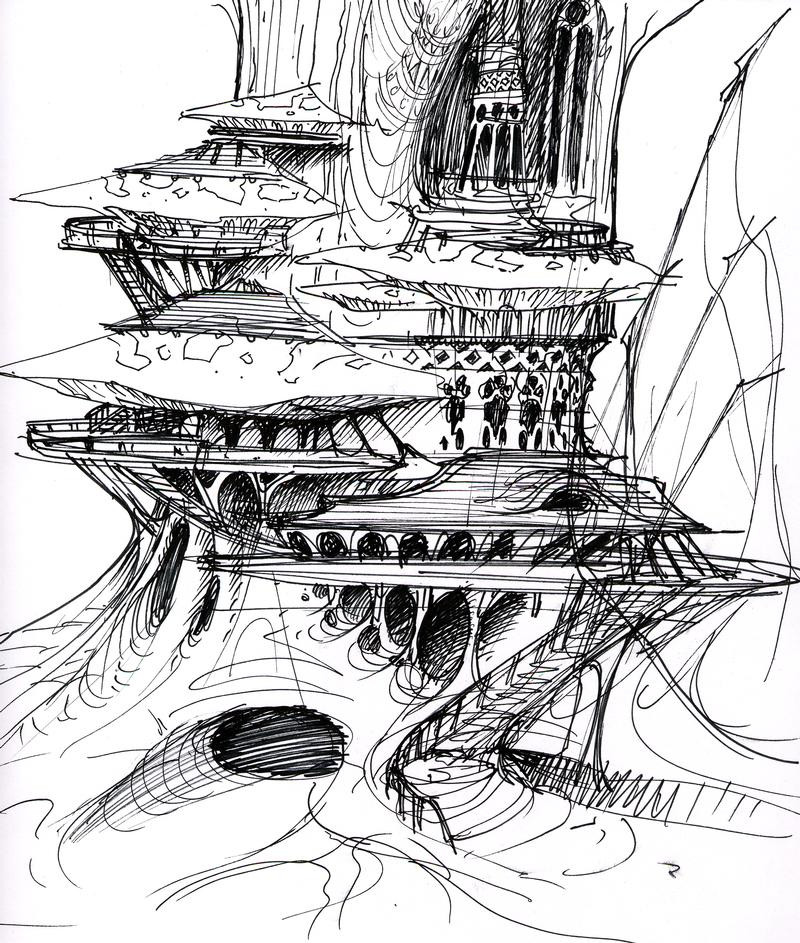
\includegraphics[scale=0.25]{./Ressources/medieval/habitation_thorneye.jpg}
\caption{Une habitation de Thorneye crayonnée par un visiteur}
\end{center}
\end{figure}
\subsubsection{Relations}
\begin{itemize}
\item Aegnord: Commerce, Très bonnes relations
\item Anksfall: Aucune relation, En paix 
\item Dren: Aucune relation, Méfiant    
\item Grahyrst: Aucune relation
\item Ketelundr: Aucune relation, Méfiant 
\item Mauhagr: Aucune relation, Inspire la peur
\item Rinam: Aucune relation, En paix 
\item Leheath:  Aucune relation, En paix 
\item Sombre-Cime: Aucune relation  
\item Vrag: Hostile
\end{itemize}
\subsection{Aegnord}
\subsubsection{Description}
\hypertarget{aegnord}{}Un des derniers royaumes elfes, cette forêt est en pleine expansion.
La ville principale est resplendissante.
Elle est habité par des elfes gris qui loge dans les racines des arbres.
Le palais royal est situé sous un chêne millénaire, tout simplement splendide.
On dit que ce chêne est à l'origine de la magie des elfes. C'est aussi le centre de la forêt.
Les elfes gris sont très pacifique et il n'ont participé à aucune guerre à ce jour. 
\subsubsection{Artisanat}
Aegnord est aussi une des vitrines de l'artisanat elfe, qui travaille l'ensemble des matériaux d'origines naturelles. Cette dague en os est un bon exemple du l'art elfe.
\begin{figure}[ht]
\begin{center}
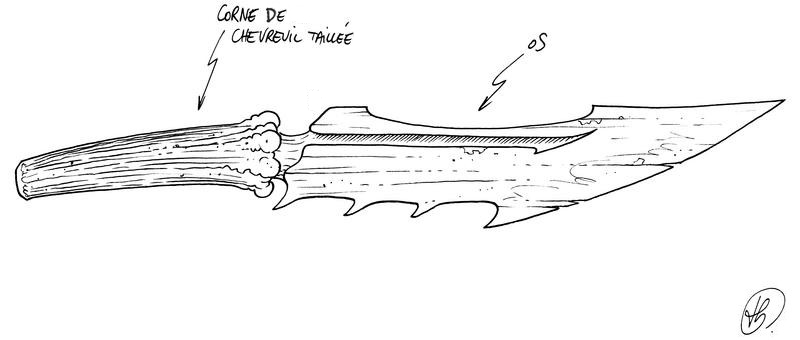
\includegraphics[scale=0.4]{./Ressources/medieval/dague_1.jpg}
\caption{Une dague en os made in Aegnord}
\end{center}
\end{figure}
\section{Les contrées barbares}
\subsubsection{Description}
\hypertarget {lescontreesbarbares}{}
Le froid, ou le l'éloignement de toute civilisation, a entrainé la séparation des ces terres du pouvoir impérial. Les humains présent ont donc commencer à s'adapter à leur milieu de vie, à tel point qu'aujourd'hui l'empire les qualifies de "barbares", bien que leur civilisation soit assez évoluée.
Les barbares sont des peuples nomades. Il n'y a donc pas de villes à proprement parler, si ce n'est d'immenses caravanes qui parcours ces steppes froides et arides.
La terre est en effet assez pauvre, mais suffisamment riche pour qu'arbustes et autres  petites plantes, ce qui attire nombre de gibier. Ces derniers constituent la base de l'alimentation des locaux, mêlées à quelques baies et végétaux récoltées en voyage.
\section{Dagat-Ys}
\subsubsection{Description}
\hypertarget {dagatys}{}Dans la langue barbare, Dagat-Ys signifie 'mer de cristal'.
En effet, cette mer n'est qu'une étendue d'eau gelée, scintillante de milles feus sous le soleil d'hiver.
Les peuplades barbares ont beaucoup de respect pour cette mer.
\subsection{Transition}
\subsubsection{Description}
\hypertarget {transition}{}
Transition est est une grande ville qui se situe dans les confins de Dagat-Ys, la mer gelée. 
Cette vile est magique. Littéralement posée sur la mer gelée, elle est d'une beauté suprême.
Durant les longs couché de soleil d'été, la lumière rouge se reflète sur la glace et produit une ambiance fantastique. Elle se construit sur une solide base rocheuse, puis monte vers le ciel.
%Croquis!
Elle est dominée par un grand palais, celui du Démiurge. Mais aucun être vivant n'y est jamais rentré.
Transition est aussi la plus grande ville de commerce d'âme. Peu de gens y habitent réellement.
Elle est surtout constituée de "gens de passage", plus ou moins long.
\subsubsection{Accès}
Pour se rendre a Transition, rien de plus simple, il suffit de se rendre dans un des chefs lieu d'une région. Une porte magique s'y trouve forcément (la plupart du temps dans les églises locales), et permet d'accéder à Transition, instantanément.
L'arrivée se fait dans la salle des portes, une grande salle circulaire dans le quartier marchand. Dans cette salle sont rassemblés l'ensemble des portails vers les grandes villes de ce monde. La milice locale y fait respecter une loi stricte.
\subsubsection{Hiérarchie}
Il n'y a ni maire, ni roi, ni prince à Transition. La ville s'auto-gère dans tous les domaines, elle possède une milice étrangement efficace.
\subsubsection{La grande maison blanche}
Transition est dominée par une grande maison blanche, à l’extrême pointe sud-ouest de la ville. La populace ne sais rien à son sujet, ni même les notables de la ville, sa présence semble normale à quiconque la contemple. Elle est là, et personne ne s'en soucie. Quelqu'un y habite sûrement. Cette maison a la particularité de ne pas avoir d'entrée. La vue que l'on a depuis les alentours de celle-ci est remarquable, et constitue un des lieux les plus impressionnant de ce monde.